\begin{figure}[htbp]

\begin{center}
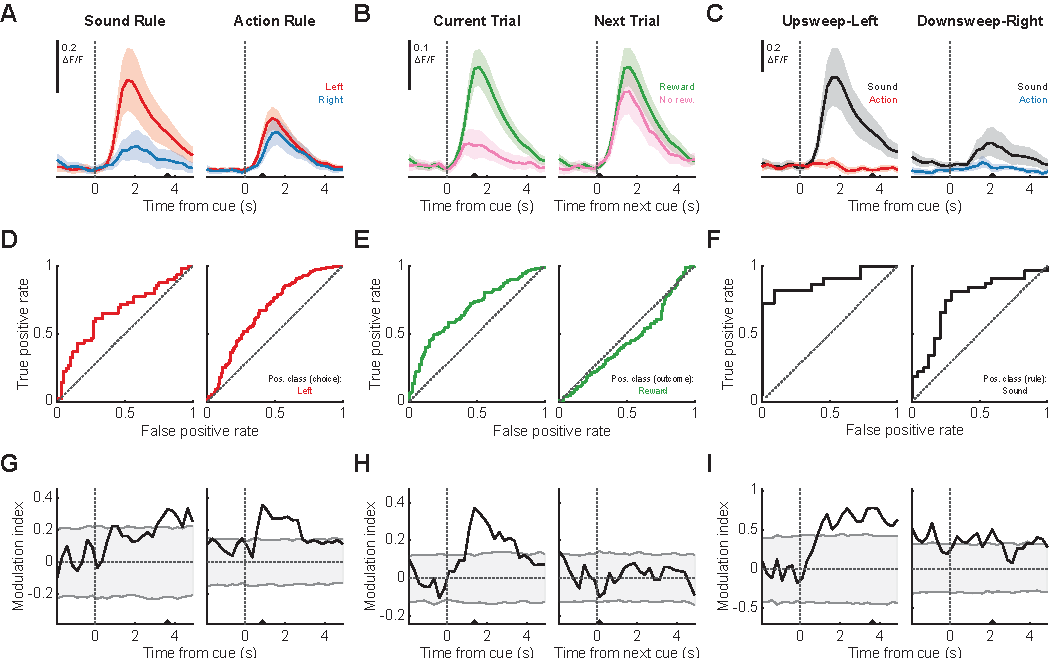
\includegraphics[width=\textwidth]{Figures/Chapter4/Fig5}
\end{center}

\caption[Example cell modulated by choice, outcome, and rule context]
{Example cell modulated by choice, outcome, and rule context. (A) Mean $\frac{\Delta F}{F}$ traces from a single PYR neuron as a function of time relative to cue onset. Traces were averaged across trials in which the left (red) or right (blue) spout was chosen. Results are presented separately for trials governed by the sound (left) and action rule (right). Shading, bootstrapped 95\% confidence intervals. (B) Mean traces associated with rewarded (green) or unrewarded choices (pink) made in the current trial. Results are plotted as a function of time relative to cue onset in the current trial (left) and the trial immediately following the indicated outcome (right). (C) Mean traces from sound vs. action trials in which the same choice was made in response to the same sound cue and resulted in a reward. Left: upsweep-left trials governed by the sound (black) or action-left rule (red). Right: downsweep-right trials governed by the sound (black) or action-right rule (blue). (D--F) Example ROC curves calculated at the time points indicated by black arrowheads in A--C. Left trials, rewarded trials, and sound trials were arbitrarily assigned positive class membership for the analysis of choice, outcome, and rule signals, respectively. (G--I) The modulation index $I$, plotted as a function of time relative to cue onset for the full series of time points in A--C. For each time $t$, $I(t)$ was calculated from the area under the corresponding ROC curve (AUC) as $2*(\mathit{AUC}-0.5)$. The shaded intervals reflect the middle 95\% of $I_{0}(t)$, a null distribution generated by replicating the analysis using shuffled class labels.}

\label{fig:Fig5}
\end{figure}